\chapter{Robinson Foulds Metric}
A field, where tree edit distances get applied a lot is the field of computational biology and bioinformatics. Comparing the structure of different RNAs is a classic example of such an application. An even more important one is comparing phylogenetic trees. A phylogenetic tree or evolutionary tree is a rooted branching diagram, that shows the evolutionary connectedness of different species. Multiple species can have recent common ancestor (in the evolutionary sense). This ancestor is represented as a node with an edge to all the descended species. A leaf is called a taxon and is labelled with the species it represents. All in all, one can build one huge phylogenetic tree that represents all life on earth. For the studies of evolutionary biology, scientists often need to compare different evolutionary theories regarding a certain subset of species. Therefore they have to take a look at the structure of the corresponding subtrees and apply some distance measurement on them. \\


\section{Additional Background}
The scientific field of phylogenetics is the field of evolutionary relationships and history among species and groups of organisms. This common ancestry is described as a phylogenetic tree. The taxons, the labels of the leaves of the phylogenetic tree, are hereby the species currently investigated. The interior nodes represent some common ancestor of the investigated species. If we create a rooted phylogenetic tree, then the root would be the common ancestor of all these species. Sometimes the structure can't be fully resolved. This results in so called \textit{multifurcations}, interior nodes of degree higher than three. 
\begin{figure}
	\centering
	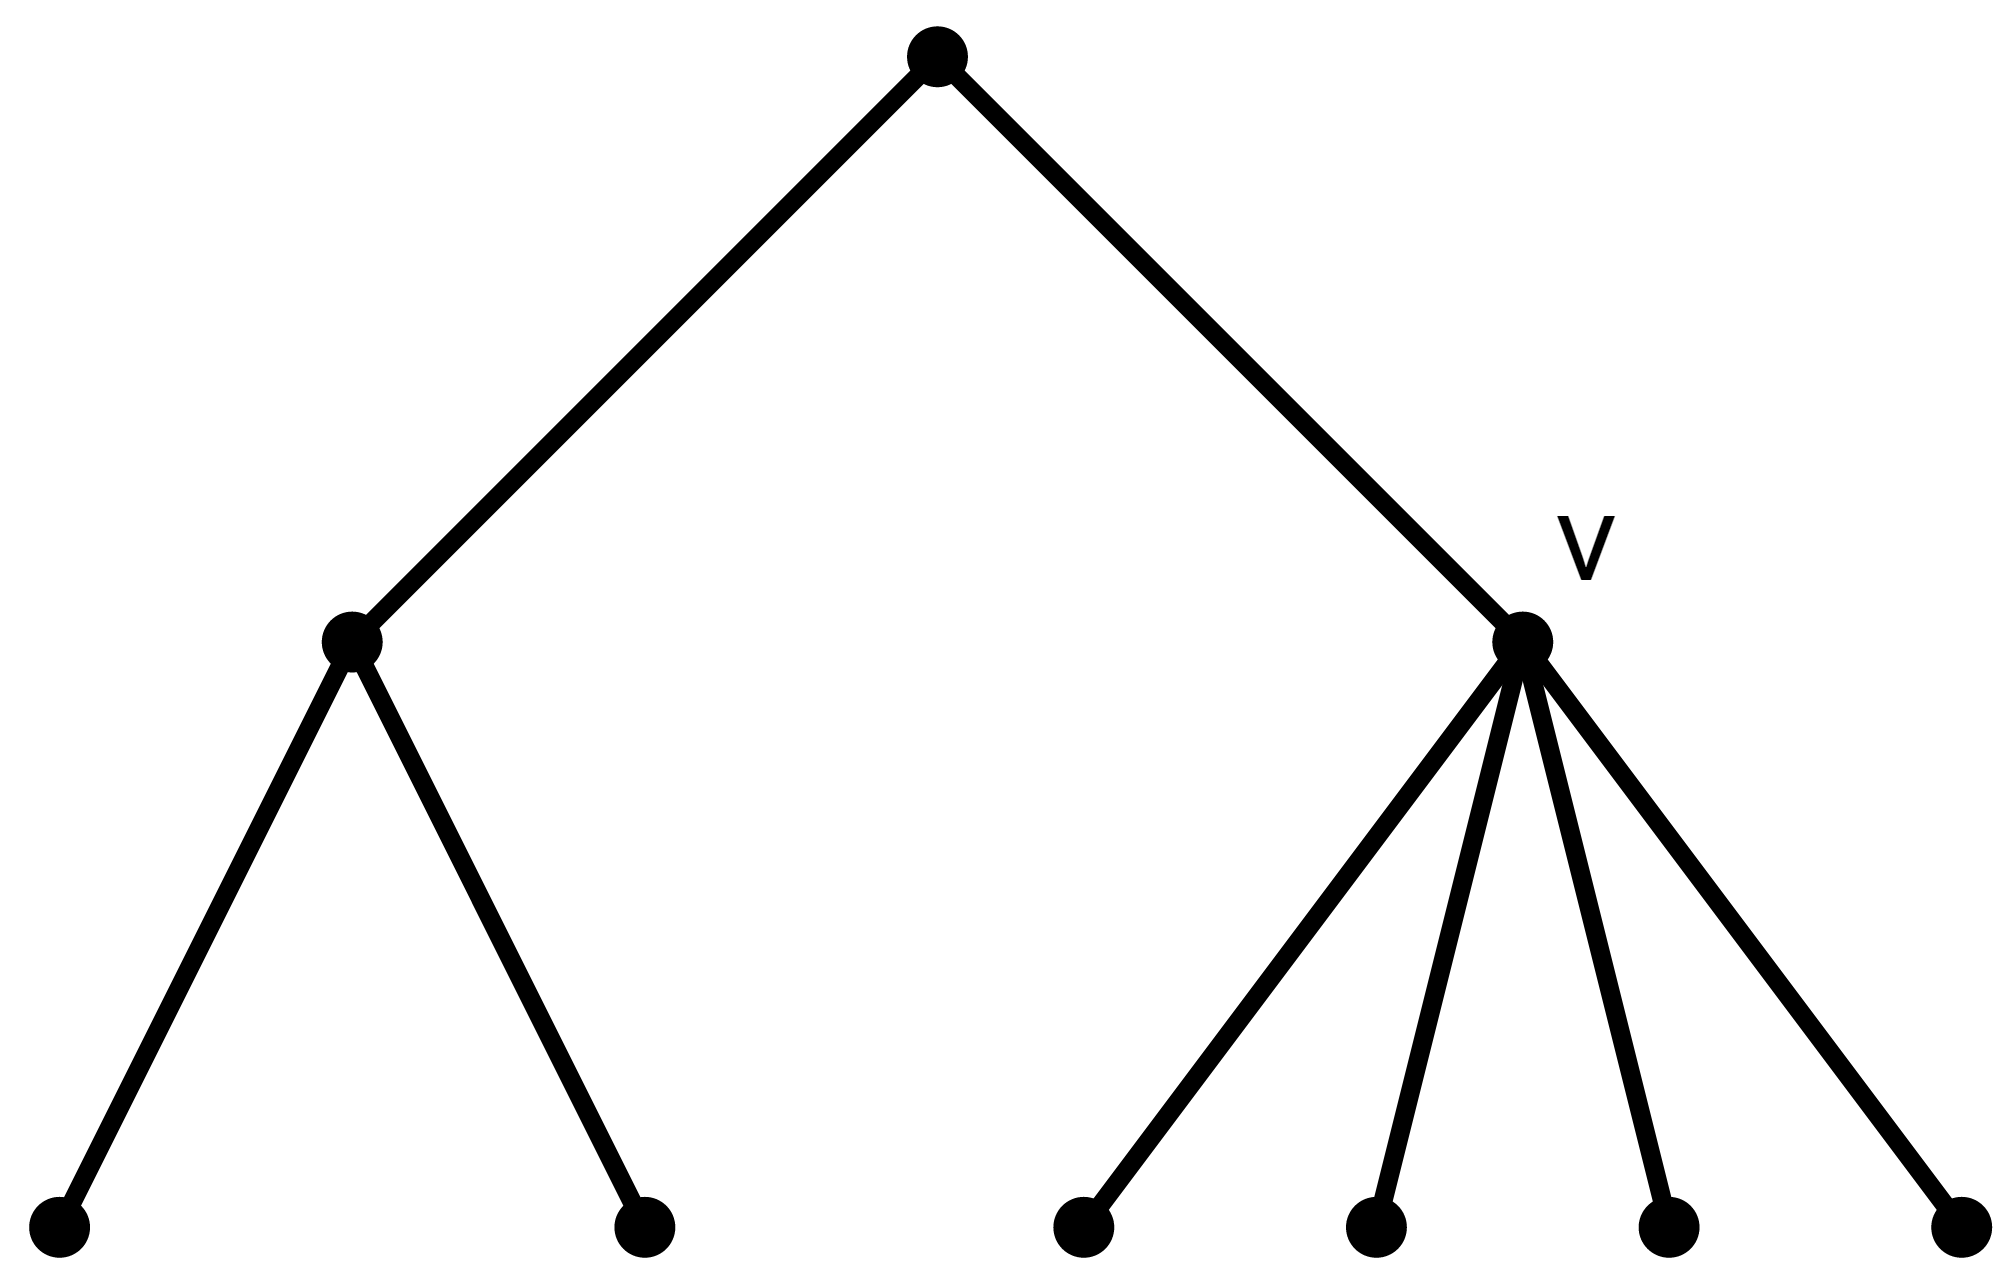
\includegraphics[width=0.4\textwidth]{figures/multifurcation.png}
    \caption{A rooted phylogenetic tree. The node $v$ is a multifurcation since its degree is larger than $3$. The ancestry relations aren't fully resolved for the children of $v$.}
\end{figure}
Multifurcations may occur due to missing data for inferring the phylogeny. Often they appear in consensus trees, when partially contradictory trees were obtained by some methods. A perfectly resolved phylogenetic tree doesn't have any multifurcations implying a binary phylogenetic tree. 

\begin{figure}
	\centering
	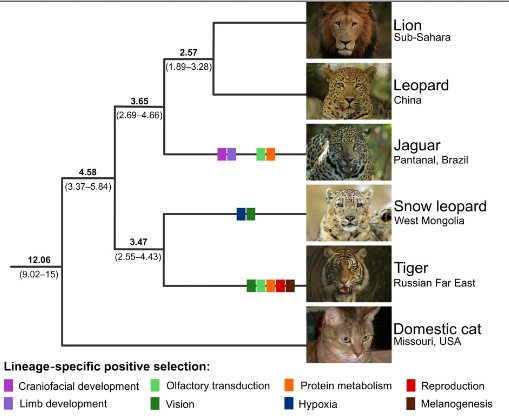
\includegraphics[width=0.4\textwidth]{figures/cats_evolution.png}
	\caption{A simplified phylogenetic tree that shows the evolutionary connection between five big cats and the domestic house cat. The complexity of finding this task is described in the paper by Figueiró et al.~\cite{Fig}.}
\end{figure}

\section{The original metric}
The most commonly used distance measurement was introduced by Robinson and Foulds~\cite{Rob}. They introduced the term \textit{clade}, which describes a group of leaves that have a common ancestor which they do not share with any other node.

The Robinson-Foulds metric is quite intuitive and easy to compute. It is the average number of non-trivial clades that are present in exactly one of the two trees:
\begin{defin}
Let $T_1,T_2$ be two trees with the same set of taxa $X$. Then we define the Robinson-Foulds metric $d_{RF}$ as follows:
\[ d_{RF} := \frac{1}{2}|\mathcal{C}^*(T_1) \bigtriangleup \mathcal{C}^*(T_2)| \]
\end{defin}
\begin{rem}
Assuming that two trees $T_1$,$T_2$ have the same set of taxa $X$ with $n:= |X|$ implies that the number of interior nodes is bounded by $n-1$ for both trees. Furthermore, since we ignore trivial clades, the clade $X$, induced by the tree's root, will be ignored. Thus we end up with a maximum RF-distance of $n-2$ for two trees with the same taxa sets of size $n$.
\end{rem}
Although the Robinson-Foulds metric is commonly used, it has some well known downsides. For example changing the position of a single leaf can yield a new tree having maximal distance from the original one. Let's take a look at Figure~\ref{fig:maxRFdist}. Let $T_1$ be the top left tree and $T_2$ be the top right one. It is easy to see that the set of clades are the following:
\begin{align*}
\mathcal{C}^*(T_1) &=\{ \{1,...,j\}\;|\;j\in \{2,...,7\}\} \\
\mathcal{C}^*(T_2) &=\{ \{2,...,j\}\;|\;j\in \{3,...,7\}\} \cup \{1,8\}
\end{align*}
Obviously in tree $T_1$ every clade contains both nodes $1$ and $2$. On the other hand in tree $T_2$ every clade either contains node $1$ or $2$, but never both of them. This implies that 
\begin{align*}
\mathcal{C}^*(T_1) \cap \mathcal{C}^*(T_2) &= \emptyset \\
d_{RF} = \frac{1}{2}|\mathcal{C}^*(T_1) \bigtriangleup \mathcal{C}^*(T_2)| &= \frac{1}{2}(|\mathcal{C}^*(T_1)| + |\mathcal{C}^*(T_2)|) \\
d_{RF} = \frac{1}{2}(6 + 6) = 6
\end{align*}
However the third tree $T_3$ also has the same RF distance of $6$ to both trees $T_1$ and $T_2$. This points to another big disadvantage of the Robinson Foulds distance. The distribution of the distances is very much concentrated on the upper end of the scale. Two arbitrary phylogenetic trees with $n$ leaves on the same set of taxa have a high probability to have a Robinson Foulds distance of $n-2$. Furthermore the example shows that the Robinson Foulds distance does not compare the structure of the two trees. Otherwise the distance between $T_1$ and $T_2$ would be much smaller than the one to the tree $T_3$. 
\begin{figure}[ht!]\label{fig:maxRFdist}
    \begin{subfigure}[b]{0.45\textwidth}
        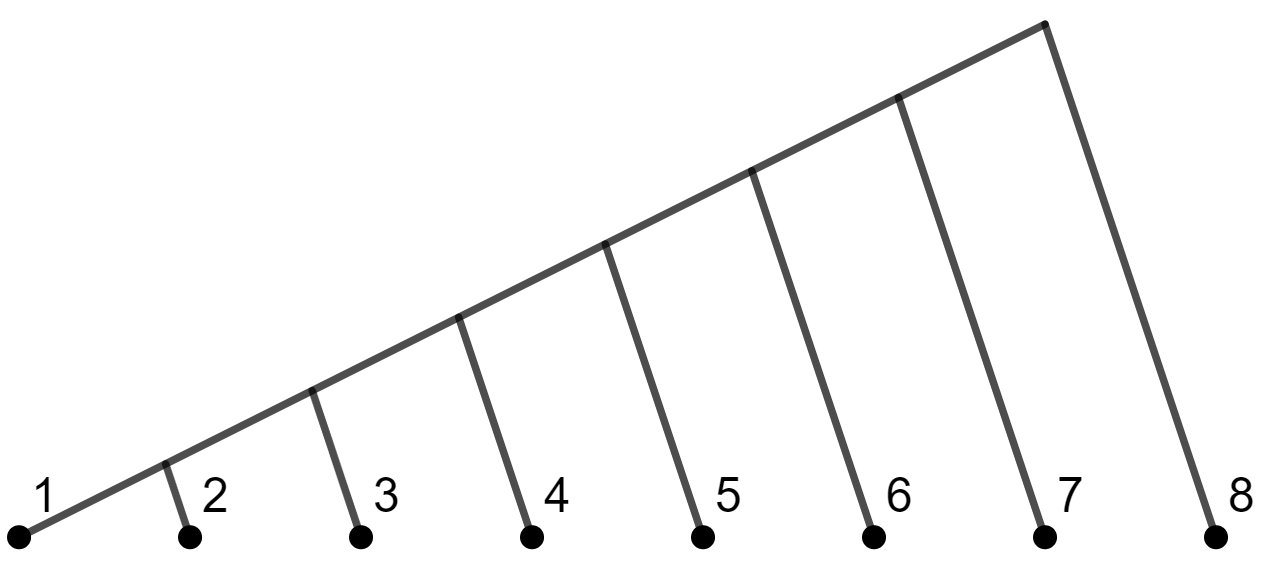
\includegraphics[width=\textwidth]{figures/RF_tree1.jpg}
    \end{subfigure}
    \quad
    \begin{subfigure}[b]{0.45\textwidth}
        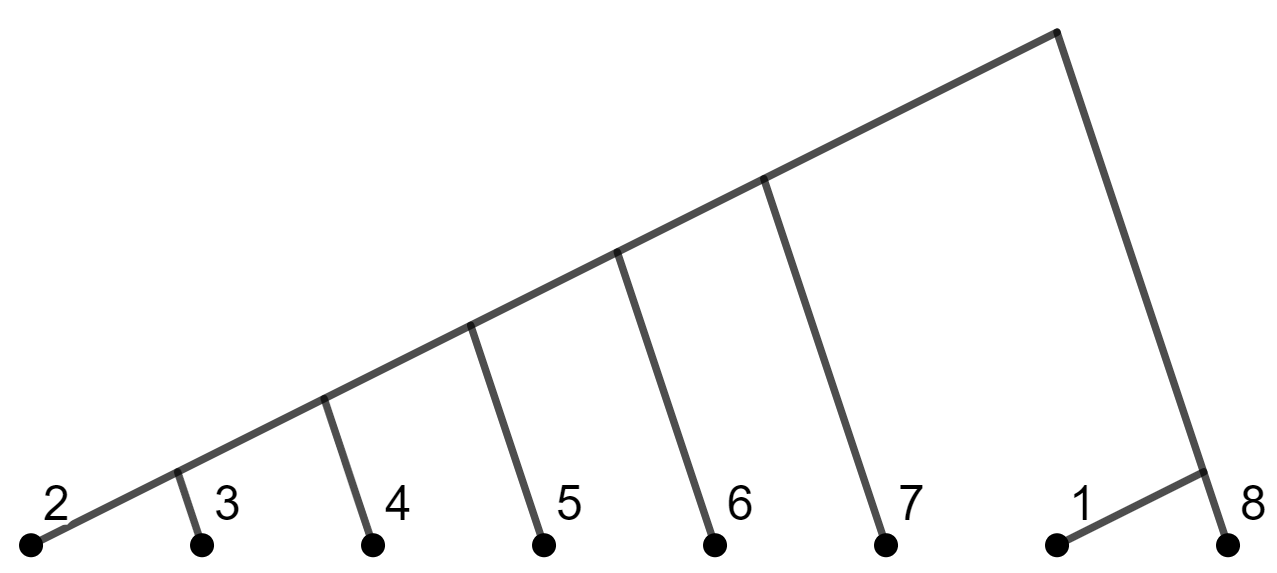
\includegraphics[width=\textwidth]{figures/RF_tree2.jpg}
    \end{subfigure}
    \quad
    \begin{subfigure}[b]{0.45\textwidth}
        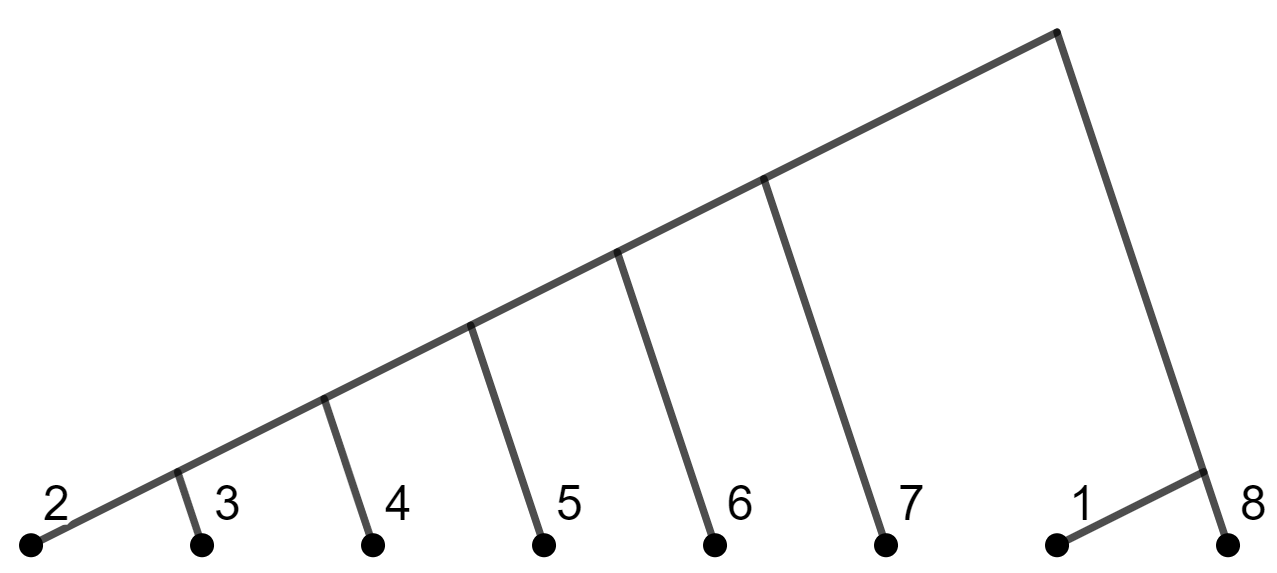
\includegraphics[width=\textwidth]{figures/RF_tree2.jpg}
    \end{subfigure}
    \caption{Three trees having the maximal RF-distance on the set of taxa $\{1,...,8\}$}
\end{figure}
 
\section{The Generalized Robinson Foulds}
To take advantage of structural similarities between $T_1$, $T_2$ Böcker et al.~\cite{Boe} suggested to extend the Robinson Foulds metric. They wanted to relax the condition of counting any clade which appears in the set of clades for one but not both trees. Therefore they introduced a bipartite graph $G(T_1, T_2)$ depending on the two trees under consideration. 
\begin{defin}\label{def:RFGraph}
Let $T_1, T_2$ be two phylogenetic trees with the same number of leaves $n$ and on the same set of taxa $X$. We define the complete bipartite graph $G_{T_1,T_2}$ on the following set of nodes:
$$G_{T_1,T_2}: \, \mathcal{C}^*(T_1) \times \mathcal{C}^*(T_2)$$
\end{defin}
\begin{defin}\label{def:RFcostfct}
Let $T_1, T_2$ be two phylogenetic trees with the same number of leaves $n$ and on the same set of taxa $X$. We introduce a cost function $\delta$ as follows:
$$\delta: \mathcal{P}(X) \times \mathcal{P}(X) \mapsto \mathcal{R}_{\geq 0} \cup \{\infty\}$$
where $\mathcal{P}(X)$ denotes the power set of $X$. The value $\delta(C,C')$ determines the dissimilarities between two clades $C$, $C' \subset X$. The value of $\delta(C, \emptyset) > 0$ denotes the dissimilarity bewtween a clade $C \in \mathcal{C}^*(T_1)$ with the empty clade in $\mathcal{C}^*(T_2)$. The value $\delta(\emptyset, C')$ is defined analogously.
\end{defin}
\begin{defin}\label{def:preRFdist}
Let $T_1, T_2$ be two phylogenetic trees with the same number of leaves $n$ and on the same set of taxa $X$. Let $G_{T_1,T_2}$ and a cost function $\delta$ be given as defined in Definitions~\ref{def:RFGraph} and~\ref{def:RFcostfct}. Furthermore let $M \subset \mathcal{C}^*(T_1) \times \mathcal{C}^*(T_2)$ be a matching in $G_{T_1,T_2}$. 
We call a clade $C \in \mathcal{C}^*(T_1)$ unmatched, if $(C, C') \notin M \; \forall C' \in \mathcal{C}^*(T_2)$, analogously for clades of $T_2$.\\
Now we can define the costs $d_{\delta}(M)$ of a matching $M$ as:
$$d_{\delta}(M) := \sum_{(C, C') \in M} \, \delta(C,C') + \sum_{\substack{C \in \mathcal{C}^*(T_1),\\ C\text{ unmatched in }M}} \delta(C, \emptyset) + \sum_{\substack{C' \in \mathcal{C}^*(T_2),\\C'\text{ unmatched in }M}} \delta(\emptyset, C')$$
Minimizing over all matchings in $G_{T_1,T_2}$ yields $\overline{d}_{\delta}(T_1,T_2)$:
$$\overline{d}_{\delta}(T_1,T_2) := \min_{M \text{ matching in }G_{T_1,T_2}} \, d_{\delta}(M)$$
\end{defin}
\begin{lem}
Let $T_1, T_2$ be two phylogenetic trees with the same number of leaves $n$ and on the same set of taxa $X$. There is a distance function $\delta_{RF}$ s.t. 
$$\overline{d}_{\delta_{RF}}(T_1,T_2) = d_{RF}(T_1,T_2)$$ 
\end{lem}
\begin{proof}
Let $\delta_{RF}: \mathcal{P}(X) \times \mathcal{P}(X) \mapsto \mathcal{R}_{\geq 0} \cup \{\infty\}$ be given as follows:
$$\delta_{RF}(C, C') = 
\begin{cases}
	0 & \text{if } C = C' \\
	\frac{1}{2} & \text{if } C = \emptyset \text{ or } C' = \emptyset \\
	\infty & \text{if } C \neq C' \text{ and } C \neq \emptyset \neq C'
\end{cases}$$
Let $M^* \subset \mathcal{C}^*(T_1) \times \mathcal{C}^*(T_2)$ be a matching s.t.:
$$\overline{d}_{\delta}(T_1,T_2) = \min_{M \text{ matching in }G_{T_1,T_2}} \, d_{\delta}(M) = d_{\delta}(M^*)$$
Since the empty matching has a finite value, $M^*$ must not contain any edge $(C, C')$ s.t. $\delta_{RF}(C, C') = \infty$. Therefore $M^*$ only contains edges where the respective clades are congruent. Thus $M^*$ minimizes the number of unmatched clades, counts them and divides this number by $2$. Thus:
$$\overline{d}_{\delta_{RF}}(T_1,T_2) =  \frac{1}{2}|\mathcal{C}^*(T_1) \bigtriangleup \mathcal{C}^*(T_2)|  = d_{RF}(T_1,T_2)$$ 
\end{proof}
\begin{lem}\label{lem:costfct}
Let $T_1, T_2$ be two phylogenetic trees with the same number of leaves $n$ and on the same set of taxa $X$. Let $G_{T_1,T_2}$ and a cost function $\delta$ be given as defined in Definitions~\ref{def:RFGraph} and~\ref{def:RFcostfct}. The task of computing the matching $M^*$ that satisfies $\overline{d}_{\delta}(T_1,T_2) = d_{\delta}(M^*)$ can be simplified by the following model:\\
For any edge $(C, C') \in E(G_{T_1,T_2})$ let its weight be given by
\begin{equation} \label{eq:costfct}
\omega(C,C') := \delta(C,\emptyset) + \delta(\emptyset, C') - \delta(C,C').
\end{equation}
Finding a minimal cost matching $M$ of clades is now equivalent to finding a maximal cost matching $M^*$ in $G_{T_1, T_2}$. \\
Furthermore, if $\delta$ is a metric, all weights are non-negative.
\end{lem}
\begin{proof}
Let $M^*$ be a maximal cost matching in $G_{T_1, T_2}$. Then the following implications are trivial:
\begin{gather*}
\sum_{\{C,C'\} \in M^*} \, \omega(C, C') = \max_{M} \, \sum_{\{C,C'\} \in M} \delta(C,\emptyset) + \delta(\emptyset, C') - \delta(C,C') \\
= \max_{M} \, \underbrace{\sum_{C \in \mathcal{C}^*(T_1)} \delta(C,\emptyset)}_{\textit{const. }K_1} - \sum_{\substack{C \in \mathcal{C}^*(T_1),\\ C\text{ unmatched}}} \delta(C,\emptyset) + \underbrace{\sum_{C' \in \mathcal{C}^*(T_2)} \delta(\emptyset, C')}_{\textit{const. }K_2} \\
- \sum_{\substack{C \in \mathcal{C}^*(T_1),\\ C\text{ unmatched}}} \delta(\emptyset, C') - \sum_{\{C,C'\} \in M} \delta(C,C')\\
= K_1 + K_2 + \max_{M} - \bigg( \sum_{\substack{C_1 \in \mathcal{C}^*(T_1),\\ C\text{ unmatched}}} \delta(C, \emptyset) + \sum_{\substack{C \in \mathcal{C}^*(T_1),\\ C\text{ unmatched}}} \delta(\emptyset, C') + \sum_{\{C,C'\} \in M} \delta(C,C') \bigg)\\
= K_1 + K_2 - \min_{M} d(M) = K_1 + K_2 - d(M^*)
\end{gather*}
Additionally, if $\delta$ is a metric, the triangle inequality holds true. Thus all all weights are non-negative.
\end{proof}
Let's compute the distances defined in Definition~\ref{def:RFcostfct} of the trees $T_1, T_2$ from Figure~\ref{fig:preRFdist} with respect to the costs of the symmetric difference between sets:
$$\delta_{sym}(C, C') = |C \triangle C'| = |C \cup C'| - |C \cap C'|$$
In this case, the best way to match a clade $\{1,...,j\} \in \mathcal{C}^*(T_1), j \geq 3$ to a clade in $\mathcal{C}^*(T_2)$ is to match it with the clade $\{2,...,j\}$, since its symmetric difference is only $1$. This handles all cases except for the clade $\{1,2\} \in \mathcal{C}^*(T_1)$ and $\{1,8\} \in \mathcal{C}^*(T_2)$. Matching those two clades is better than keeping them unassigned, since:
$$\delta_{sym}(\{1,2\},\{1,8\}) = 2 < 4 = \delta_{sym}(\{1,2\},\emptyset) + \delta_{sym}(\emptyset, \{1,8\})$$
Resulting in a matching of overall costs of $8$. 

Another way to compute the distance is to use Lemma~\ref{lem:costfct}. In Figure~\ref{fig:maxCostMatch} we can investigate the graph $G_{T_1,T_2}$ with the corresponding edge weights.
\begin{figure}
	\centering
	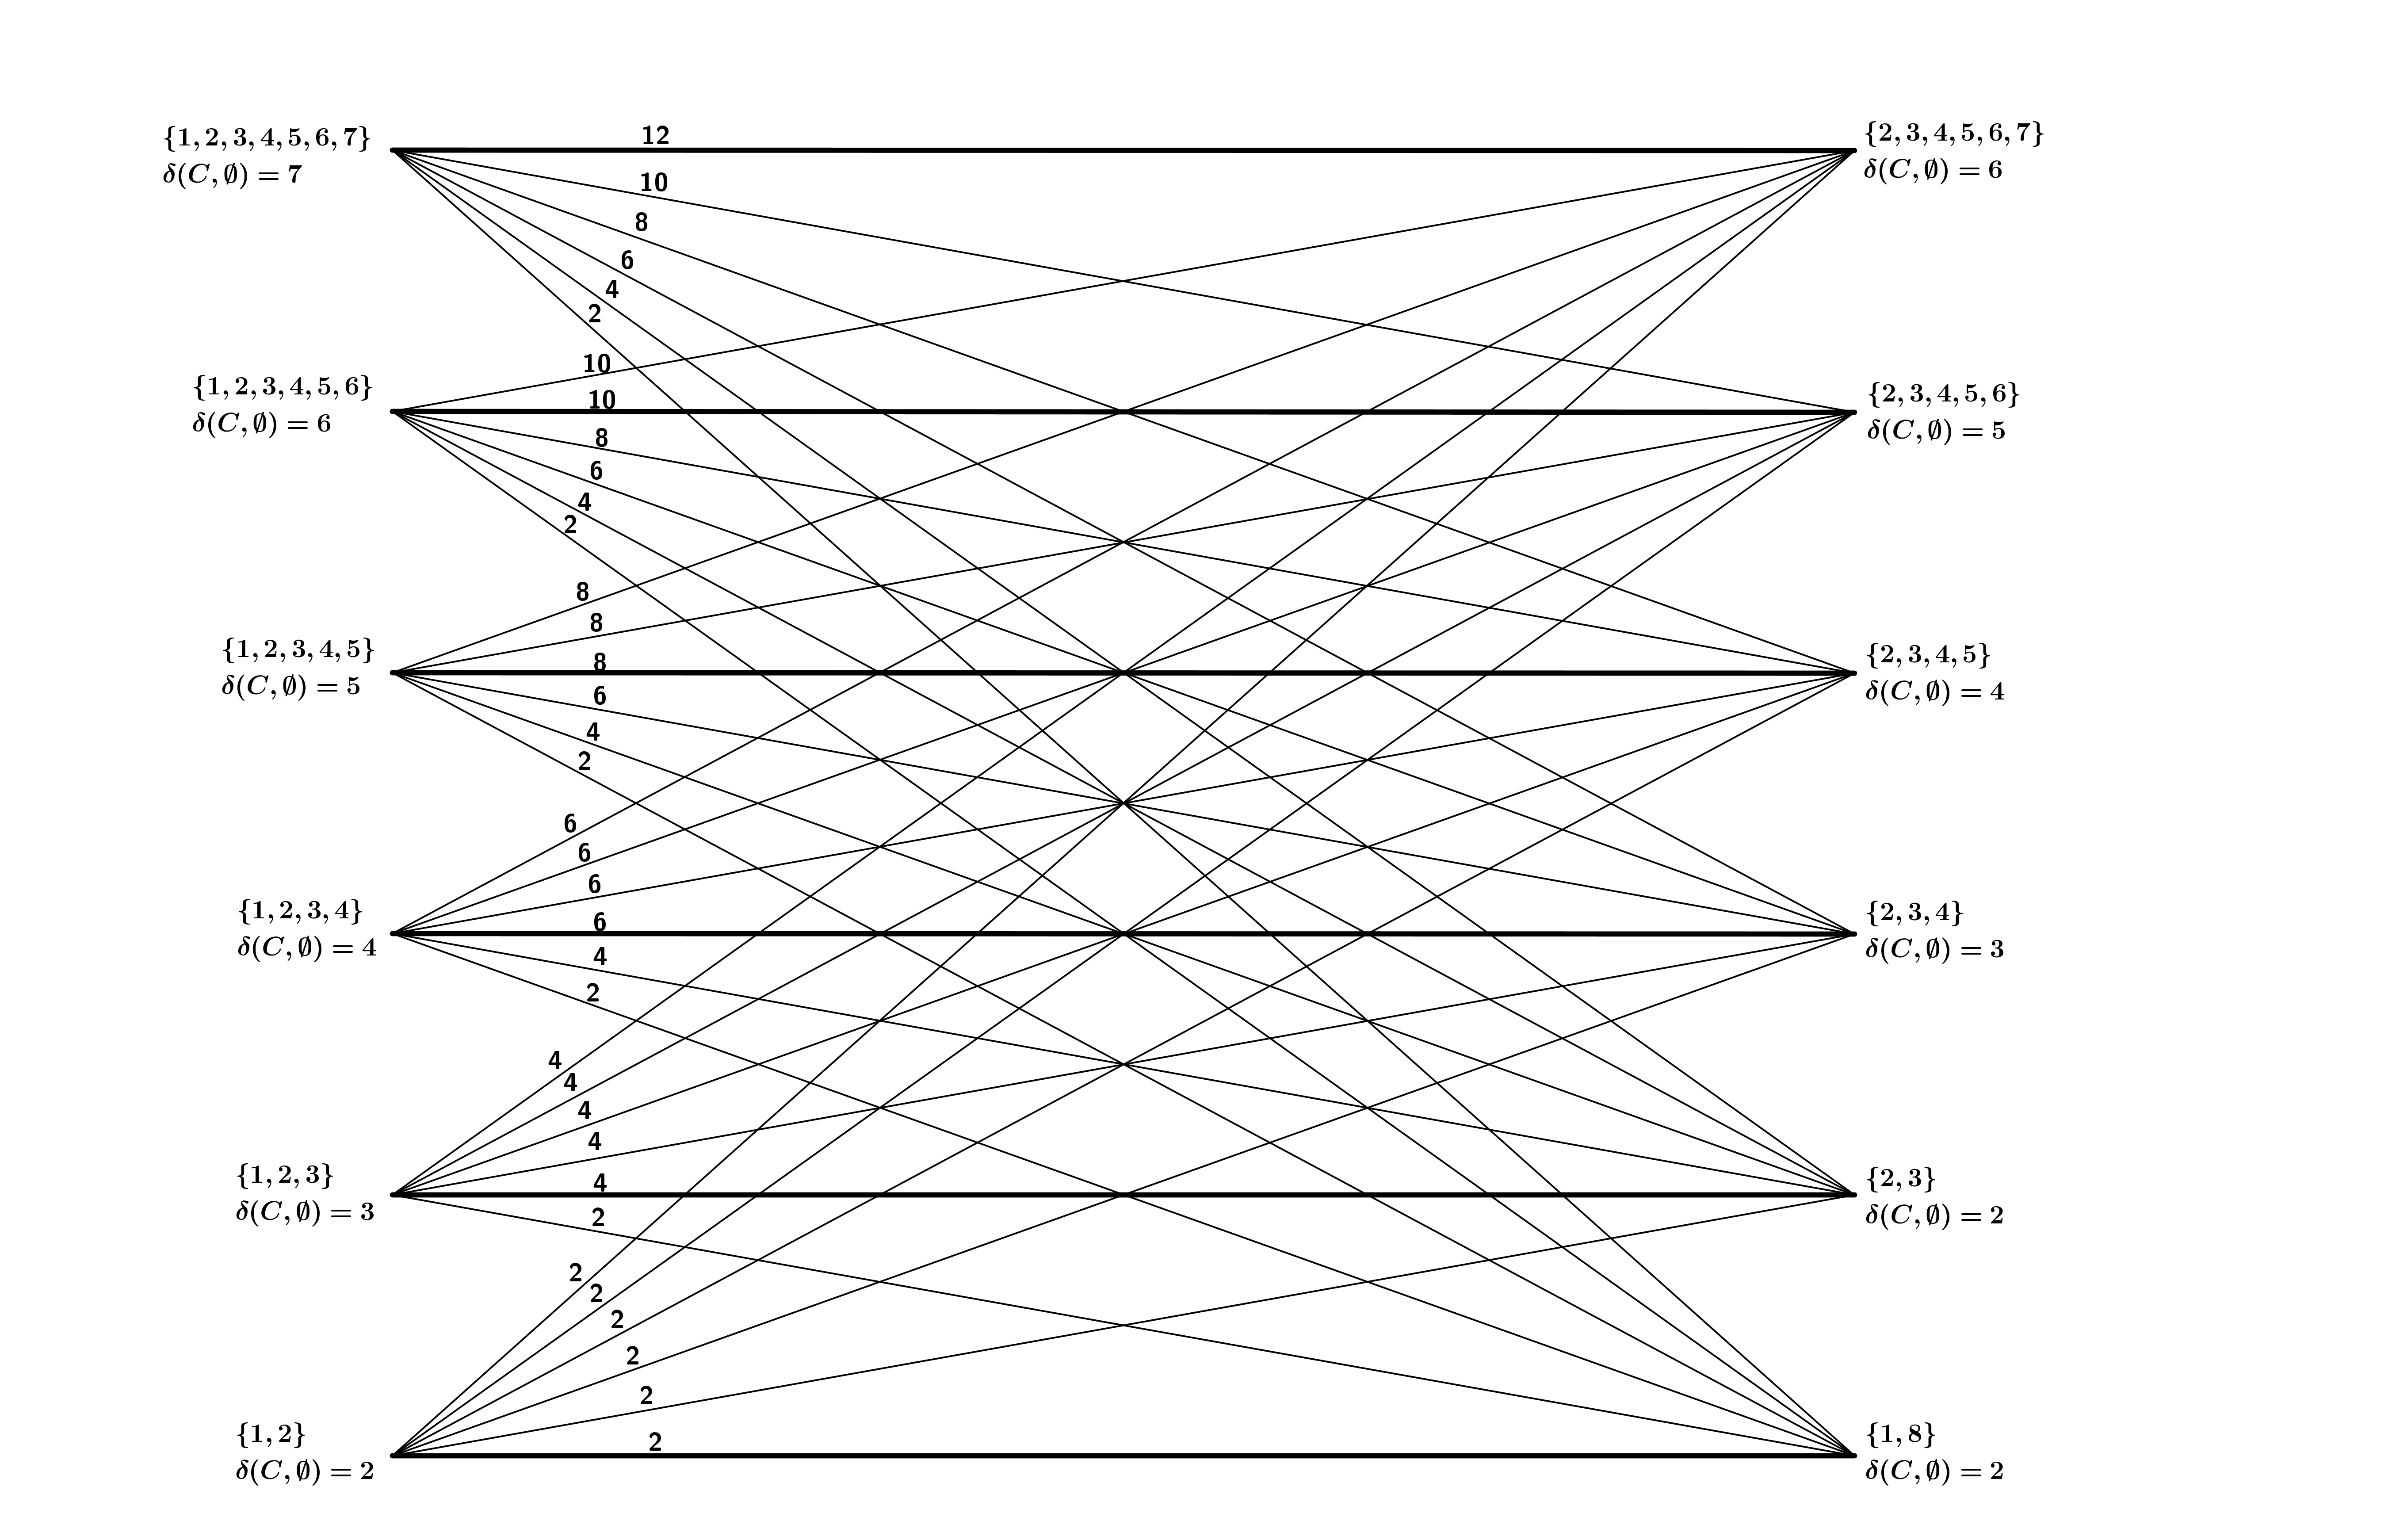
\includegraphics[width=1.25\textwidth]{figures/maxCostMatching.png}
    \caption{This is the graph $G_{T_1,T_2}$. On the left hand side we see nodes corresponding to the non-trivial clades of $T_1$, on the right hand side nodes corresponding to the ones of $T_2$. The edges of $G_{T_1,T_2}$ have their weights assigned. The maximum cost matching $M^*$ is represented by the bold edges.}
\end{figure} 
The optimal matching in $G_{T_1,T_2}$ can be seen very easily. For every edge $(C_1,C_2)$ in the matching $M^*$, the weight $\omega(C_1,C_2)$ is maximal among all edges starting at $C_1$. Thus $M^*$ indeed is optimal.

Now let's compare this distance to the distance of $T_1$ and $T_2$ to $T_3$ respectively:
\begin{align*}
\bar{d}_{\delta_{sym}}(T_1, T_2) &= 8\\
\bar{d}_{\delta_{sym}}(T_1, T_3) &= 19\\
\bar{d}_{\delta_{sym}}(T_2, T_3) &= 16
\end{align*}
This distance measure delivers values which are nearer to the observers intuitive answers. The distances indicate significant similarities between the trees $T_1$ and $T_2$. Furthermore they point out that $T_3$ has a completely different structure than the other trees.\\
Of course the values can only be compared with distances with respect to the same cost function $\delta$. Generally, comparing the distances $\overline{d}_{\delta}(T_1,T_2)$ and $\bar{d}_{\delta'}(T_1,T_2)$ is not unfeasible without adding any context. For example comparing $\bar{d}_{\delta_{RF}}(T_1,T_2) = 6 < 8 = \bar{d}_{\delta_{sym}}(T_1, T_2)$ doesn't yield any information. However one can get information from the follwoing inequalities:
\begin{align*}
6 = \delta_{RF}(T_1,T_2) = \delta_{RF}(T_1,T_3) =\delta_{RF}(T_2,T_3) = 6 \\
8 = \bar{d}_{\delta_{sym}}(T_1, T_2) < 16 = \bar{d}_{\delta_{sym}}(T_2, T_3) < \bar{d}_{\delta_{sym}}(T_1, T_3) &= 18
\end{align*}
The minimum matching for $\bar{d}_{\delta_{sym}}(T_1, T_2)$ shown above demonstrates a problem with this straight forward approach: The clade $\{1,2\} \in \mathcal{C}^*(T_1) \subset \{1,...,j\} \in \mathcal{C}^*(T_1) \forall j \geq 3$, however this doesn't hold for its matched clade $\{1,8\}$. Therefore we need to concentrate on arboreal matchings:

\begin{defin}\label{def:arboreal}
Let two rooted phylogenetic trees $T_1, T_2$ on the same set of taxa $X$ be given. A matching $M$ on their sets of non-trivial clades is called \textit{arboreal} if for any two edges $\{C_1,C_2\}, \{C_1',C_2'\} \in M$ one of the following cases hold:
\begin{enumerate}
\item $C_1 \subseteq C_1' \wedge C_2 \subseteq C_2'$
\item $C_1' \subseteq C_1 \wedge C_2' \subseteq C_2$
\item $C_1 \cap C_1' = \emptyset \wedge C_2 \cap C_2' = \emptyset$
\end{enumerate}
\end{defin}
\begin{defin}
Let $T_1$ and $T_2$, two rooted phylogenetic trees on the same set of taxa $X$, and a cost function $\delta$ be given. We define $d_{\delta}(T_1,T_2)$ as follows:
$$d_{\delta}(T_1,T_2) = \min_{\substack{M \text{ matching in }G_{T_1,T_2} \\ M \text{ arboreal}}} \, d_{\delta}(M)$$
We denote the value $d_{\delta}(T_1,T_2)$ as the \textit{generalized Robinson-Foulds distance} between $T_1$ and $T_2$ with respect to $\delta$.
\end{defin} 
\begin{rem}
Some notes about the generalized Robinson-Foulds distance:
\begin{enumerate}
\item From now on we will abbreviate the generalized Robinson-Foulds distance with \textbf{gRF}.
\item The gRF $d_{\delta}(T_1,T_2)$ and the previous distance measure $\overline{d}_{\delta}(T_1,T_2)$ are very similar. The only difference is, that the gRF minimizes over the arboreal matchings only.
\item The inequality $\overline{d}_{\delta}(T_1,T_2) \leq d_{\delta}(T_1,T_2)$ trivially holds.
\item Lemma~\ref{lem:costfct} also holds for the gRF $d_{\delta}(T_1,T_2)$. The proof works the same way, but instead of maximizing over all matchings, we only consider arboreal ones.
\end{enumerate}
\end{rem}
\begin{lem}
Let $X$, a set of taxa, and a cost function $\delta$ be given. Furthermore assume $\delta$ to be a metric. Then the gRF with respect to $\delta$ is a metric on the set of rooted phylogenetic trees on $X$.
\end{lem}
The proof is provided in the full version of the Böcker et al.'s paper~\cite{Boe}.

\subsection{Jaccard-Robinson-Foulds metric}
One specific metric used as a cost function is motivated by the Jaccard index of two sets: 
$$J(A,B) = \frac{|A \cap B|}{|A \cup B|}$$
Generalizing this idea leads to the Jaccard weights of order $k$:
\begin{align}\label{eq:JacWeights}
\delta_k(C_1,C_2) = 
\begin{cases}
0 & \text{if } C_1 = C_2 = \emptyset \\
1 - (\frac{|C_1 \cap C_2|}{|C_1 \cup C_2|})^k & \text{else}
\end{cases}
\end{align}
\begin{lem} \label{lem:kron}
Let $\delta_k(C_1,C_2)$ be given as defined in Equation~(\ref{eq:JacWeights}). Then $\delta_k(C_1,C_2)$ converge to the inverse Kronecker delta as $k \to \infty$:
$$\delta_k(C_1,C_2) =
\begin{cases}
0 & \text{if } C_1 = C_2 \\
1 & \text{if } C_1 \neq C_2
\end{cases}$$
\end{lem}
\begin{proof}
\textbf{Case 1}: $C_1 = C_2$.\\
\begin{align*}
\delta_k(C_1,C_2) = 1 - (\frac{\overbrace{|C_1 \cap C_2|}^{|C_1|}}{\underbrace{|C_1 \cup C_2|}_{|C_1|}})^k = 1 - (1)^k = 0 \; \forall k \in \mathbb{N}
\end{align*}
\textbf{Case 2}: $C_1 \neq C_2$
\begin{align*}
&\Rightarrow (C_1 \cup C_2) \setminus (C_1 \cap C_2) \neq \emptyset \\
&\Rightarrow |C_1 \cup C_2| > |C_1 \cap C_2| \\
&\Rightarrow \frac{|C_1 \cap C_2|}{|C_1 \cup C_2|} < 1 \\
&\Rightarrow (\frac{|C_1 \cap C_2|}{|C_1 \cup C_2|})^k \underset{k \to \infty}{\to} 0 \\
&\Rightarrow \delta_k(C_1,C_2) = 1 - (\frac{|C_1 \cap C_2|}{|C_1 \cup C_2|})^k \underset{k \to \infty}{\to} 1 \\
\end{align*}
\end{proof}
\begin{defin}
Let $T_1$ and $T_2$, two rooted phylogenetic trees on the same set of taxa $X$ and a positive $k \, \in \, \mathbb{R}_{\geq 0}$ be given. The induced gRF metric is called Jaccard-Robinson-Foulds metric (\textbf{JRF}) of order $k$ and is denoted by $d_{JRF}^{(k)}(T_1,T_2)$.\\
\end{defin}
\begin{thm}
The JRF of order $k$ converges to the Robinson-Foulds distance as $k \to \infty$.
\end{thm}
\begin{proof}
For a fixed problem, there is only a finite number of non-trivial clades. Every Jaccard-distance tends to the inverse Kronecker delta as stated in Lemma~\ref{lem:kron}. Therefore the following holds:
\begin{align*}
\forall \, 0 < q < 1: \exists \, K \in \mathbb{N} \; \text{s.t.} \forall \, k > K:\\
 \delta_k(C_1,C_2) 
 \begin{cases} 
 = 0 &\text{ if }C_1 = C_2 \\
 = 1 &\text{ else if } C_1 = \emptyset \text{ or } C_2 = \emptyset\\
 > 1-q &\text{ else if } C_1 \neq C_2
 \end{cases}
\end{align*}
Let $M$ be a matching that minimizes $d_{RF}(T_1,T_2)$. 
\begin{align*}
&d_{RF}(M) - d_{JRF}^{(k)}(M) =\\
&\sum_{(C, C') \in M} \, (\delta_{RF}(C,C') - \delta_{JRF}^{(k)}(C,C')) + \sum_{\substack{C \in \mathcal{C}^*(T_1),\\ C\text{ unmatched in }M}} (\overbrace{\delta_{RF}(C, \emptyset)}^{=1} - \overbrace{\delta_{JRF}^{(k)}(C, \emptyset)}^{=1}) \\
&+ \sum_{\substack{C' \in \mathcal{C}^*(T_2),\\C'\text{ unmatched in }M}} (\overbrace{\delta_{RF}(\emptyset, C')}^{=1} - \overbrace{\delta_{JRF}^{(k)}(\emptyset, C')}^{=1}) = \\
&\sum_{\substack{(C, C') \in M \\ C = C'}} \, (\overbrace{\delta_{RF}(C,C')}^{=0} - \overbrace{\delta_{JRF}^{(k)}(C,C')}^{=0}) + \sum_{\substack{(C, C') \in M \\ C \neq C'}} \, (\overbrace{\delta_{RF}(C,C')}^{=1} - \overbrace{\delta_{JRF}^{(k)}(C,C'))}^{> 1-q} < \\
& \sum_{\substack{(C, C') \in M \\ C \neq C'}} q < n*q \underset{q \rightarrow 0}{\rightarrow} 0 
\end{align*}
\end{proof}

\subsection{Computational Complexity}
In their paper Böcker et al. demonstrate a polynomial reduction from the $(3,4)$-SAT problem to the problem of finding a minimal cost arboreal matching, even if the cost function $\delta$ is a metric. The $(3,4)$-SAT is the problem of finding a satisfying assignment for a Boolean formula in which every clause consists of exactly $3$ literals and any variable occurs $4$ times.\\
The authors of the above mentioned paper were able to construct a minimum arboreal matching instance $I$ for any Boolean formula $\phi \in (3,4)$-SAT. If the problem $I$, using the symmetric difference as cost function, admits a solution with a value smaller than a certain value, the original problem of finding a correct assignment for $\phi$ has a solution. For more details we suggest to read the original paper~\cite{Boe}. 
\begin{thm}
For an instance of the arboreal matching using the symmetric difference as cost function $\delta$ and an integer $k$, it is $NP$-complete whether there exists an arboreal matching of cost at most $k$.
\end{thm}

\subsection{An Integer Linear Program}
One way to approach an $\mathcal{NP}$-complete problem is to formulate it as an integer linear program and solve the latter. Therefore Böcker et al. set up an integer linear programming formulation to find a minimum cost arboreal matching.\\
Let two rooted phylogenetic trees $T_1 = (V_1,E_1)$ and $T_2 = (V_2,E_2)$ and a cost function $\delta: \mathcal{C}(T_1 \times \mathcal{C}(T_2) \mapsto \mathbb{R}_{\geq 0}$ be given. We number the clades in $\mathcal{C}(T_i)$ from $1$ to $|V_i|$ for $i \in \{1,2\}$. Then the indicator variable $x_{i,j}$ represents whether the $i$-th clade $C_i$ in $\mathcal{C}(T_1)$ is matched with the $j$-th clade $C'_j$ in $\mathcal{C}(T_2)$. We use the cost function introduced in Equation~(\ref{eq:costfct}) to find a minimum cost matching while maximizing the sum of the cost function. To recapitulate, the value for $\omega(C_i,C'_j)$ is:
$$\omega(C_i,C'_j) = \delta(C_i,\emptyset) + \delta(\emptyset, C'_j) - \delta(C_i,C'_j)$$
We also have to make sure that the assignment we receive satisfies the conditions for an arboreal matching. Therefore we introduce the set $\mathcal{I}$ with the following properties:
\begin{equation*}
\mathcal{I} := \bigg\{ \{(i,j), (k,l)\} \, \Big| \, \parbox{9.8cm}{The edges $(C_i, C'_j)$ and $(C_k, C'_l)$ violate the conditions
\\for arboreal matchings defined in Definition~\ref{def:arboreal}} \bigg\}
\end{equation*}
\begin{thm}\label{thm:gRF_LP}
Let $T_1$ and $T_2$, two rooted phylogenetic trees on the same set of taxa $X$, and a cost function $\delta$ be given. Furthermore let a fixed order of all non-trivial clades in $\mathcal{C}(T_1)$ and $\mathcal{C}(T_2)$ and the cost function $\omega(C_i,C_j')$ be given. We introduce a linear integer problem with decision variables $x_{i,j}$ as follows.
\begin{align}
\max &\sum_{i=1}^{|V_1|} \sum_{j=1}^{|V_2|} \; \omega(C_i, C'_j) x_{i,j} \label{eq:max} \\
\text{s.t.} &\sum_{j=1}^{|V_2|} \; x_{i,j} \leq 1 & \forall i \in \{1,...,|V_1|\} \label{eq:V_1} \\
&\sum_{i=1}^{|V_1|} \; x_{i,j} \leq 1 & \forall j \in \{1,...,|V_2|\} \label{eq:V_2} \\
&x_{i,j} + x_{k,l} \leq 1 & \forall \{(i,j), (k,l)\} \in \mathcal{I} \label{eq:arb} \\
&x_{i,j} \in \{0,1\} & \forall i \in \{1,...,|V_1|\}, \forall j \in \{1,...,|V_2|\} \label{eq:int}
\end{align}
Let $x^*_{i,j}$ be the values of the indicator variables $x_{i,j}$ of an optimal solution of the linear integer problem. Let $M^*$ be the following set of edges:
$$(C_i,C_j') \, \in \, M^* \quad \Leftrightarrow \quad x^*_{i,j} = 1$$
Then the set of edges $M^*$ is a matching that realizes the value of the gRF:
$$d_{\delta}(T_1, T_2) = d_{\delta}(M^*)$$
\end{thm}
\begin{proof}Here we sketch the proof of the equivalence between the linear integer program~(\ref{eq:max}) - (\ref{eq:int}) and the minimum cost arboreal matching problem.\\
First and foremost, the restriction to integer decision variables in Equation~(\ref{eq:int}) ensures, that we either choose an edge to be in the matching or not. Thus we indeed get a set of edges. Furthermore Equations~(\ref{eq:V_1}) and~(\ref{eq:V_2}) restricts the chosen set of edges to be a (not necessarily complete) matching. Last but not least, because of Equation~(\ref{eq:arb}) we can be certain that the matching we end up with is a an arboreal matching, since we constructed the set $\mathcal{I}$ exactly this way. As proven in Lemma~\ref{lem:costfct}, the arboreal matching of maximum cost with respect to the cost function~(\ref{eq:max}) is an arboreal matching that minimizes the gRF $d_{\delta}(T_1, T_2)$.
\end{proof}